
\begin{frame}

\begin{tabular}{lll}
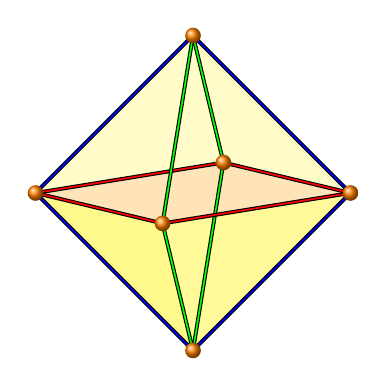
\begin{tikzpicture}[scale=2,z=-5.5]
  \tikzset{VertexStyle/.style = {shape          = circle,
                                 ball color     = orange,
                                 text           = black,
                                 inner sep      = 2pt,
                                 outer sep      = 0pt,
                                 minimum size   = 4 pt}}
  \tikzset{EdgeStyleRed/.style   = {thin,
                                 double          = red}}
%                                 double distance = 1pt}}
  \tikzset{EdgeStyleBlue/.style   = {thin,
                                 double          = blue}}
%                                 double distance = 1pt}}
  \tikzset{EdgeStyleGreen/.style   = {thin,
                                 double          = green}}
%                                 double distance = 1pt}}


\coordinate (A1) at (0,0,-1);
\coordinate (A2) at (-1,0,0);
\coordinate (A3) at (0,0,1);
\coordinate (A4) at (1,0,0);
\coordinate (B1) at (0,1,0);
\coordinate (C1) at (0,-1,0);


\draw [fill opacity=0.7,fill=yellow!30] (A2) -- (A3) -- (B1) -- cycle;
\draw [fill opacity=0.7,fill=yellow!30] (A3) -- (A4) -- (B1) -- cycle;
\draw [fill opacity=0.9,fill=yellow!50] (A2) -- (A3) -- (C1) -- cycle;
\draw [fill opacity=0.8,fill=yellow!50] (A3) -- (A4) -- (C1) -- cycle;
\draw [fill opacity=0.7,fill=orange!30] (A2) -- (A3) -- (A4) -- (A1)-- cycle;

\draw[EdgeStyleRed] (A1) -- (A2);
\draw[EdgeStyleRed] (A2) -- (A3);
\draw[EdgeStyleRed] (A4) -- (A1);
\draw[EdgeStyleBlue] (A2) -- (B1);
\draw[EdgeStyleGreen] (A1) -- (B1);
\draw[EdgeStyleGreen] (A3) -- (B1);
\draw[EdgeStyleBlue] (A4) -- (B1);
\draw[EdgeStyleBlue] (A2) -- (C1);
\draw[EdgeStyleGreen] (A1) -- (C1);
\draw[EdgeStyleGreen] (A3) -- (C1);
\draw[EdgeStyleBlue] (A4) -- (C1);
\draw[EdgeStyleRed] (A3) -- (A4);

\draw (A1)  node[VertexStyle]  {};
\draw (A2)  node[VertexStyle]  {};
\draw (A3)  node[VertexStyle]  {};
\draw (A4)  node[VertexStyle]  {};
\draw (B1)  node[VertexStyle]  {};
\draw (C1)  node[VertexStyle]  {};


\end{tikzpicture}
&&
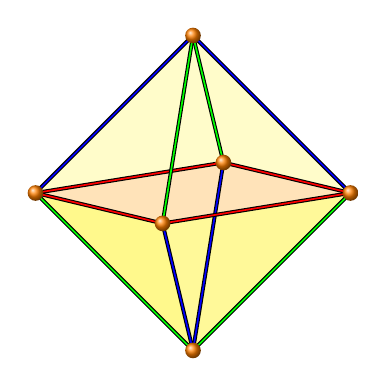
\begin{tikzpicture}[scale=2,z=-5.5]
  \tikzset{VertexStyle/.style = {shape          = circle,
                                 ball color     = orange,
                                 text           = black,
                                 inner sep      = 2pt,
                                 outer sep      = 0pt,
                                 minimum size   = 4 pt}}
  \tikzset{EdgeStyleRed/.style   = {thin,
                                 double          = red}}
%                                 double distance = 1pt}}
  \tikzset{EdgeStyleBlue/.style   = {thin,
                                 double          = blue}}
%                                 double distance = 1pt}}
  \tikzset{EdgeStyleGreen/.style   = {thin,
                                 double          = green}}
%                                 double distance = 1pt}}


\coordinate (A1) at (0,0,-1);
\coordinate (A2) at (-1,0,0);
\coordinate (A3) at (0,0,1);
\coordinate (A4) at (1,0,0);
\coordinate (B1) at (0,1,0);
\coordinate (C1) at (0,-1,0);


\draw [fill opacity=0.7,fill=yellow!30] (A2) -- (A3) -- (B1) -- cycle;
\draw [fill opacity=0.7,fill=yellow!30] (A3) -- (A4) -- (B1) -- cycle;
\draw [fill opacity=0.9,fill=yellow!50] (A2) -- (A3) -- (C1) -- cycle;
\draw [fill opacity=0.8,fill=yellow!50] (A3) -- (A4) -- (C1) -- cycle;
\draw [fill opacity=0.7,fill=orange!30] (A2) -- (A3) -- (A4) -- (A1)-- cycle;

\draw[EdgeStyleRed] (A1) -- (A2);
\draw[EdgeStyleRed] (A2) -- (A3);
\draw[EdgeStyleRed] (A4) -- (A1);
\draw[EdgeStyleBlue] (A2) -- (B1);
\draw[EdgeStyleGreen] (A1) -- (B1);
\draw[EdgeStyleGreen] (A3) -- (B1);
\draw[EdgeStyleBlue] (A4) -- (B1);
\draw[EdgeStyleGreen] (A2) -- (C1);
\draw[EdgeStyleBlue] (A1) -- (C1);
\draw[EdgeStyleBlue] (A3) -- (C1);
\draw[EdgeStyleGreen] (A4) -- (C1);
\draw[EdgeStyleRed] (A3) -- (A4);

\draw (A1)  node[VertexStyle]  {};
\draw (A2)  node[VertexStyle]  {};
\draw (A3)  node[VertexStyle]  {};
\draw (A4)  node[VertexStyle]  {};
\draw (B1)  node[VertexStyle]  {};
\draw (C1)  node[VertexStyle]  {};
\end{tikzpicture}\\
\quad
\quad
$mmm$-octahedron & & 
\quad
\quad
$rmm$-octahedron
\end{tabular}
\end{frame}

